\documentclass[conference]{IEEEtran}
\IEEEoverridecommandlockouts
% The preceding line is only needed to identify funding in the first footnote. If that is unneeded, please comment it out.
\usepackage{cite}
\usepackage{amsmath,amssymb,amsfonts}
\usepackage{algorithmic}
\usepackage{graphicx}
\usepackage{textcomp}
\usepackage{xcolor}
\usepackage{svg}
\usepackage{amsmath}
\usepackage{multirow}
\usepackage{rotating}

\usepackage{mdframed}
\usepackage{hyperref}
\usepackage{tikz}
\usepackage{makecell}
\usepackage{tcolorbox}
\usepackage{amsthm}
\usepackage{float}

%\usepackage[english]{babel}
\usepackage{pifont} % checkmarks
%\theoremstyle{definition}
%\newtheorem{definition}{Definition}[section]


\usepackage{listings}
\lstset
{ 
    basicstyle=\footnotesize,
    numbers=left,
    stepnumber=1,
    xleftmargin=5.0ex,
}


%SCJ
\usepackage{subcaption}
\usepackage{array, multirow}
\usepackage{enumitem}
\usepackage{lipsum}


\def\BibTeX{{\rm B\kern-.05em{\sc i\kern-.025em b}\kern-.08em
    T\kern-.1667em\lower.7ex\hbox{E}\kern-.125emX}}
\begin{document}

%\IEEEpubid{978-1-6654-8356-8/22/\$31.00 ©2022 IEEE}
% @Sune:
% Found this suggestion: https://site.ieee.org/compel2018/ieee-copyright-notice/
% I have added it - you can see if it fulfills the requirements

%\IEEEoverridecommandlockouts
%\IEEEpubid{\makebox[\columnwidth]{978-1-6654-8356-8/22/\$31.00 ©2022 IEEE %\hfill} \hspace{\columnsep}\makebox[\columnwidth]{ }}
                                 %978-1-6654-8356-8/22/$31.00 ©2022 IEEE
% copyright notice added:
%\makeatletter
%\setlength{\footskip}{20pt} 
%\def\ps@IEEEtitlepagestyle{%
%  \def\@oddfoot{\mycopyrightnotice}%
%  \def\@evenfoot{}%
%}
%\def\mycopyrightnotice{%
%  {\footnotesize 978-1-6654-8356-8/22/\$31.00 ©2022 IEEE\hfill}% <--- Change here
%  \gdef\mycopyrightnotice{}% just in case
%}

      
\title{Developing Industry 4.0 systems with a focus on Quality Attributes and Microservice Architecture\\
}

\author{
    \IEEEauthorblockN{
        Bence Boros\IEEEauthorrefmark{1},
        Botond Füzi\IEEEauthorrefmark{1},
        Edvinas Andrijauskas\IEEEauthorrefmark{1},
        Miroslav Zniscinskij\IEEEauthorrefmark{1},
        Sabina Elena Baghiu\IEEEauthorrefmark{1}
    }
    \IEEEauthorblockA{
        University of Southern Denmark, SDU Software Engineering, Odense, Denmark \\
        Email: \IEEEauthorrefmark{1} \textnormal{\{bebor23,bofuz23,eandr23,mizni23,sabag23\}}@student.sdu.dk
    }
}



%%%%

%\author{\IEEEauthorblockN{1\textsuperscript{st} Blinded for review}
%\IEEEauthorblockA{\textit{Blinded for review} \\
%\textit{Blinded for review}\\
%Blinded for review \\
%Blinded for review}
%\and
%\IEEEauthorblockN{2\textsuperscript{nd} Blinded for review}
%\IEEEauthorblockA{\textit{Blinded for review} \\
%\textit{Blinded for review}\\
%Blinded for review \\
%Blinded for review}
%\and
%\IEEEauthorblockN{3\textsuperscript{nd} Blinded for review}
%\IEEEauthorblockA{\textit{Blinded for review} \\
%\textit{Blinded for review}\\
%Blinded for review \\
%Blinded for review}
%}

%%%%
%\IEEEauthorblockN{2\textsuperscript{nd} Given Name Surname}
%\IEEEauthorblockA{\textit{dept. name of organization (of Aff.)} \\
%\textit{name of organization (of Aff.)}\\
%City, Country \\
%email address or ORCID}



\maketitle
\IEEEpubidadjcol
\begin{abstract}

In response to the complexities of Industry 4.0, this project undertakes the task of architecting and implementing prototype for mineral water bottle production system components. With a keen focus on interoperability, availability, and continuous deployability, our aim is to design a flexible system capable of seamless information exchange among different production components.  The anticipated outcome include prototype demonstrating the effective interaction of different services , databases and communication protocols, providing valuable insights into the complex decisions made during the design process. This project  seeks to establish a robust foundation for the evolution of Industry 4.0 production systems, adapting flexibility and effectiveness to meet the dynamic demands of evolving manufacturing needs. 

\begin{IEEEkeywords}
    Microservice architecture, Quality Attributes, Industry 4.0,
\end{IEEEkeywords}
\end{abstract}

\section{Introduction and Motivation}
%Introduction and motivate the problem


\emph{Introduction.}
In the ever-evolving landscape of manufacturing, the mineral water production industry stands at the intersection of tradition and technological innovation. Traditional approaches to equipment maintenance, often characterized by fixed schedules or reactive responses to failures, have proven to be inefficient, resulting in increased downtime, higher maintenance costs, and an elevated risk of unforeseen breakdowns. In the pursuit of operational excellence, there is a compelling need to explore transformative solutions that align with the principles of Industry 4.0.

\emph{Motivation.}
Efficiency is the crucial in any production sector, where the demand for seamless production processes is heightened by consumer expectations and market competition. The motivation for this research stems from the recognition that the prevalent maintenance paradigms fall short of meeting the industry's dynamic demands. Unplanned downtime can disrupt production cycles and lead to financial setbacks. To address these challenges, the motivation is to delve into the realm of predictive maintenance strategies, leveraging the advancements brought about by Industry 4.0.

The key motivation lies in reshaping the maintenance landscape, moving from scheduled interventions to a predictive model that anticipates and mitigates potential failures. By embracing Industry 4.0 technologies, such as IoT devices, automation, and data analytics, the goal is to not only enhance operational efficiency but also to enter in a new era of cost-effective and proactive maintenance practices. This research seeks to contribute valuable insights that empower mineral water production facilities to navigate the complexities of modern manufacturing, ensuring a continuous and optimized production flow. As we embark on this exploration, the aim is to lay the groundwork for a paradigm shift that aligns maintenance strategies with the dynamic needs of Industry 4.0, ultimately adopting a resilient and forward-looking mineral water production system.
 
\section{Problem and Approach}

\label{sec:problem}
\emph{Problem.}
In traditional manufacturing settings, equipment maintenance is often performed on a fixed schedule or in reaction to failures. This approach can lead to unnecessary downtime, increased maintenance costs, and a higher risk of unexpected breakdowns. In mineral water production, where efficiency is crucial, minimizing downtime and optimizing maintenance activities are essential.  


In the realms of Industry 4.0 the main challenge lies in ensuring seamless availability, interoperability and effective communication among diverse components. Integrating various programming languages, frameworks, and technologies adds complexity, each bringing its unique advantages and trade-offs.

This paper aims to identify architectural patterns that leverage best practices to address this challenge. By exploring associated advantages and constraints, the goal is to propose a unified solution for robust and resilient systems.

\newblock 

\emph{Research questions:}
\begin{enumerate}
    \item How chosen architecture design support a production system requirements?
    \item Which architectural trade-offs must be taken due to the technology choices? 
\end{enumerate}

\newblock 

\emph{Approach.}
The following steps are taken to answer this paper's research questions: 
\begin{enumerate}
    \item Develop a comprehensive system architecture that prioritizes interoperability, availability, and continuous deployability
    \item Build and implement the prototype, integrating different components of the mineral water bottle production system.
    \item Conduct simulations or real-world testing to validate the effectiveness of the prototype in facilitating seamless information exchange
\end{enumerate}

\newblock 

\section{Related work}
\label{sec:related_work}


The systematic literature review undertaken in this study explores the current state of research in Industry 4.0 production systems, with a specific focus on mineral water production \cite{Ali2023}. The review encompasses a comprehensive search strategy employing the ScienceDirect academic database, utilizing key search terms such as "Industry 4.0," "Mineral Water," and "Smart Manufacturing" \cite{Soori2023}.

The inclusion and exclusion criteria were carefully defined to ensure relevance to Industry 4.0 and technological advancements \cite{Soori2023}. The review's findings are organized into four key themes: Integration of IoT, Automation and Robotics, Big Data Analytics, and Sustainability \cite{Soori2023}.

These themes represent significant trends in the adoption of Industry 4.0 principles in manufacturing, particularly in the context of mineral water production \cite{Ali2023} \cite{Morgan2021}. The Integration of IoT is identified as a major trend, emphasizing the extensive use of IoT devices equipped with sensors to monitor and control various aspects of the production process \cite{Soori2023}.

Automation and Robotics are highlighted as transformative elements, with a focus on Reconfigurable Manufacturing Systems (RMS) \cite{Morgan2021}. Examples of RMS applications, such as reconfigurable robots and modular processes, showcase the potential to manage and automate complex and customized manufacturing processes \cite{Morgan2021}.

Big Data Analytics is recognized as a significant aspect of Industry 4.0 adoption, providing in-depth data exploration for a better understanding of manufacturing processes \cite{Berges2021}. The challenges of developing software tools for customized data analysis and visualization are acknowledged, with a mention of a semantic-based visual query system bridging the gap between manufacturing experts and IT professionals \cite{Berges2021}.

Sustainability is a key focus in the context of mineral water production, with Industry 4.0 technologies playing a vital role \cite{Bai2020}. Advanced ICT solutions, including Blockchain and Artificial Intelligence, coupled with smart concepts like smart metering and demand response, contribute to sustainable management of water supply systems \cite{Bai2020}\cite{Grigoras2018}. The potential for achieving significant energy and cost savings aligns with the global shift toward eco-friendly manufacturing practices \cite{Bai2020}.

In the discussion section, the synthesis of these findings emphasizes the transformative impact of Industry 4.0 technologies on mineral water production \cite{Ali2023}\cite{Morgan2021}\cite{Bai2020}. The use of IoT devices, automation, big data analytics, and sustainability practices collectively reshape the industry, fostering efficiency and environmentally conscious production processes\cite{Ali2023}\cite{Soori2023}\cite{Bai2020}.

This systematic literature review contributes to the field by providing a comprehensive overview of the integration of Industry 4.0 technologies in mineral water production \cite{Ali2023}. The synthesis of findings highlights key trends, challenges, and opportunities, offering valuable insights for researchers, practitioners, and industry stakeholders \cite{Ali2023}\cite{Soori2023}\cite{Bai2020}. The contextualization of this study within the existing state of the art underscores its contribution to advancing knowledge in the field of smart manufacturing and Industry 4.0 applications in the specific domain of mineral water production \cite{Ali2023}\cite{Soori2023}.


\section{Use Case and Quality Attribute Scenario}
\label{sec:use_case_and_qas}

\subsection{Use Case}
\label{sec:use_case}
\subsubsection{\textbf{Produce Order}}

The use case presents process from order initiation to successful production 

\begin{table}[H]
    \centering
    \begin{tabular}{|l|p{0.7\linewidth}|}
        \hline
        \textbf{Use Case Name} & Produce Order \\
        \hline
        \textbf{Description} & The system manages and fulfills customer orders by orchestrating various stages of order processing, initiated by a customer request. \\
        \hline
        \textbf{Primary Actor} & System \\
        \hline
        \textbf{Preconditions} & A customer request is made, and the project manager provides necessary order details (customer name, amount, mineral water bottle size). \\
        \hline
        \textbf{Main Flow} & \\
        1. & Project manager inserts order details: customer name, amount, and selects mineral water bottle size. \\
        2. & System receives and stores order information. \\
        3. & System transmits the order to the scheduler. \\
        4. & System requests necessary resources from supply \\
        5. & System receives required resources. \\
        6. & Order placed inside the queue. \\
        7. & System accepts order and initiates the production line process. \\
        8. & Project manager is informed about current state of the production proce. \\
        \hline
        \textbf{Alternative Flow} & \\
        A1. & SSystem notifies insufficient resources. \\
        A2. & System notifies the product manager to reevaluate the order. \\
        \hline
        \textbf{Postconditions} & The order is successfully processed and fulfilled. \\
        \hline
        \textbf{Exceptions} & None \\
        \hline
        \textbf{Notes} & This use case outlines the systematic process of managing and fulfilling customer orders, ensuring a seamless flow from order initiation to production. \\
        \hline
    \end{tabular}
    \caption{Use Case: Produce Order}
\end{table}


\subsection{Quality Attribute Scenarios}
\label{sec:qas}


\subsubsection{\textbf{Interoperability}}The System needs to integrate with a new third-party logistics provider to expand the supply chain network.

\begin{table}[H]
    \centering
    \begin{tabular}{|l|p{0.6\linewidth}|}
        \hline
        \textbf{Attribute} & \textbf{Outcome} \\
        \hline
        \textbf{Source of Stimulus:} & External System Integrator or third-party applications. \\
        \hline
        \textbf{Stimulus:} & New integration requirements or updates to existing interfaces. \\
        \hline
        \textbf{Environment:} & The system is actively processing orders. \\
        \hline
        \textbf{Artifact:} & Interfaces and communication protocols between the system and external systems. \\
        \hline
        \textbf{Response:} & The system should seamlessly integrate with the new logistics provider's through APIs, ensuring data exchange compatibility and smooth collaboration in order processing. \\
        \hline
        \textbf{Response Measure:} & Measure the time and success rate of integrating with new systems or updates, ensuring minimal downtime and successful data transfer. \\
        \hline
    \end{tabular}
    \caption{Interoperability QAS}
\end{table}

\subsubsection{\textbf{Availability}}Production software must run 24/7

\begin{table}[H]
    \centering
    \begin{tabular}{|l|p{0.6\linewidth}|}
        \hline
        \textbf{Attribute} & \textbf{Outcome} \\
        \hline
        \textbf{Source of Stimulus:} & Continuous monitoring or health-check system. \\
        \hline
        \textbf{Stimulus:} & Detection of system unavailability or performance degradation. \\
        \hline
        \textbf{Environment:} & The system is in production, and customer orders are actively being processed. \\
        \hline
        \textbf{Artifact:} & The entire system, including servers, databases, and critical services. \\
        \hline
        \textbf{Response:} & The system should be designed and configured to ensure continuous operation, allowing for the processing of orders at any time of the day or night. \\
        \hline
        \textbf{Response Measure:} & Measure the time it takes for the system to recover from an outage or performance degradation, ensuring that the system maintains 24/7 availability with minimal downtime. \\
        \hline
    \end{tabular}
    \caption{Availability QAS}
\end{table}

\subsubsection{\textbf{Continuous Deployability}}Production software must be continuously deployable

\begin{table}[H]
    \centering
    \begin{tabular}{|l|p{0.6\linewidth}|}
        \hline
        \textbf{Attribute} & \textbf{Outcome} \\
        \hline
        \textbf{Source of Stimulus:} & Continuous Integration/Continuous Deployment (CI/CD) pipeline or development team. \\
        \hline
        \textbf{Stimulus:} & New code changes or feature updates are ready for deployment. \\
        \hline
        \textbf{Environment:} & Development, staging, or production environment. \\
        \hline
        \textbf{Artifact:} & Codebase and configuration files. \\
        \hline
        \textbf{Response:} & The system should support continuous integration and deployment practices, allowing for the seamless roll out of new features without disrupting ongoing order processing. \\
        \hline
        \textbf{Response Measure:} & Measure the time and success rate of deploying new changes, ensuring that updates can be seamlessly integrated without disrupting the order fulfillment process. \\
        \hline
    \end{tabular}
    \caption{Continuous Deployability QAS}
\end{table}


\section{solution}
\label{sec:middleware_architecture}
The design of the system architecture is crucial to achieving the stated Quality Attribute Scenarios (QASes) outlined in the previous section. This section will delve into the proposed design that aims to ensure interoperability, availability, and continuous deployability of the system.

The designed architecture consists of five services with different programming languages and frameworks, two databases and various communication mechanisms including message broker. All of components are containerized through Docker and managed using Docker Compose. The system architecture diagram can be seen in Figure \ref{fig:system-architecture}. The communication between system components is illustrated in the Sequence diagram \ref{fig:sequence-diagram} found in Appendix A

\begin{figure}[h]
    \centering
    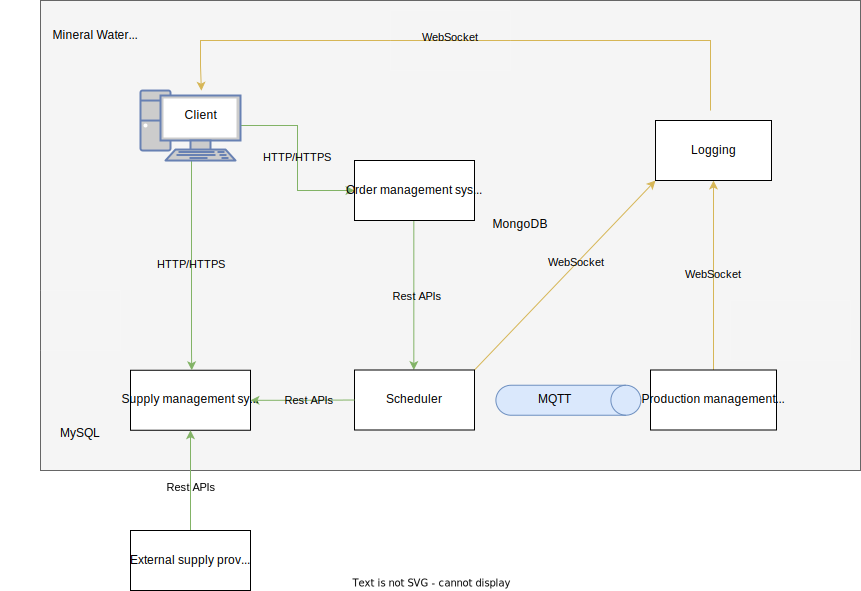
\includegraphics[width=1\linewidth]{diagrams/architecture-diagram.png}
    \caption{System architecture diagram}
    \label{fig:system-architecture}
\end{figure}

\subsection{Services}
\label{sec:services}
\begin{itemize}
    \item Order management system (OMS) (C\#/ASP.NET)
    \item Production management system (PMS) (Python)
    \item Supply management system (SMS) (Java/Spring)
    \item Scheduler (Python)
    \item Logging (JavaScript/Node.js)
    \item Dashboard/Client (JavaScript/React)
\end{itemize}

\subsection{Databases}
\label{sec:databases}
\begin{itemize}
    \item MongoDB (used by order management system to store orders)
    \item MySQL (used by supply management system to store resources)
\end{itemize}

\subsection{Communication mechanisms}
\label{sec:communication-mechanisms}
\begin{itemize}
    \item MQTT (Mosquitto message broker)
    \item RestAPI
    \item WebSocket
\end{itemize}

To ensure availability, the system employs a robust monitoring strategy, utilizing a logging system that actively sends logs through websockets from multiple components. This proactive approach enables real-time fault detection, complemented by exception handling in critical areas of the production process to facilitate graceful recovery from faults.

Deployability is enhanced through a well-managed deployment pipeline, incorporating script deployment stages with various commands for linting, artifact uploading, testing, building, and pushing images. Git and GitHub Actions workflows are utilized for version control, continuous integration, and deployment management, ensuring a streamlined CI/CD process with effortless rollback capabilities.

Interoperability holds a pivotal role, especially in collaborations with external partners. The system architecture is deliberately crafted to facilitate seamless communication between the enterprise and external entities. The utilization of a microservices approach enables autonomous scaling and modification of services, catering to evolving business requirements. Despite introducing intricacies, advanced interfaces, and rigorous testing, this approach guarantees the system's adaptability and continuous availability. The system's structure is intentionally designed with modularity and scalability in mind, ensuring efficient handling of customer orders. The architecture embraces microservices to amplify flexibility and maintainability. Each microservice is dedicated to specific functionalities, such as order management, supply management, and production management.

To serve to diverse requirements and components, different programming languages are employed for various microservices within the system. For instance, C\# was used for order management due to its simplicity, while Java was chosen for resource-intensive tasks in supply management. This multilingual approach allows leveraging the strengths of each language for specific functionalities.
However, potential drawbacks include increased complexity and maintenance challenges associated with multiple programming languages.

The system adopts a diverse persistence approach, utilizing MySQL for the supply management system and MongoDB for the order management system. flyway, a reliable database migration tool, was employed specifically for the MySQL database to ensure seamless migration and version control. This strategic use of technologies addresses the unique data storage needs of each microservice, leveraging the strengths of MySQL's reliability and MongoDB's flexibility. The incorporation of flyway streamlines database management, mitigating challenges associated with evolving schemas. While managing multiple database technologies introduces complexity, the tailored solutions enhance performance and scalability for each microservice.

Point-to-point communication between microservices is facilitated through a combination of HTTP/REST APIs and WebSockets, Mosquitto message broker. HTTP/REST APIs are utilized for synchronous communication, enabling microservices to request and respond to each other's services. WebSocket and Mosquitto message broker are employed for asynchronous communication, allowing real-time updates while reducing response time. Mosquitto, an MQTT (Message Queuing Telemetry Transport) broker, facilitates lightweight and efficient communication, especially suitable for scenarios where low latency and minimal overhead are crucial. This ensures reliable asynchronous communication and decoupling of services.

Containerization was implemented using Docker and Docker Compose to allow define and manage the services comprising the system. Each individual service had build Docker image inside CI/CD pipeline that would be push to Github Container Registry. Docker Compose simplified the orchestration and deployment of multiple containers, ensuring consistency across different environments, including development (local) and production (deployed to VM). However, approach using might to be suitable to make application completetly scalable as docker compose only allows to deploy to a single server. Better approach would be using Docker Swarm or more advanced scaling tool like K8s (Kubernetes) to manage containers deployed across multiple nodes. [14]

The Observer Pattern is applied in the system to handle situations where the Supply Management System notifies about insufficient resources. In this scenario, the Order Management System acts as the subject, and the Supply Management System serves as the observer. This pattern enables efficient communication and notification of changes in resource availability, allowing the system to dynamically respond to shortages. 
 
\section{Evaluation}
\label{sec:evaluation}

This Section describes the evaluation of the proposed design.
Section \ref{sec:design} introduces the design of the experiment to evaluate the system.
Section \ref{sec:measurements} identifies the measurements in the system for the experiment.
Section \ref{sec:pilot_test} describes the pilot test used to compute the number of replication in the actual evaluation. 
Section \ref{sec:analysis} presents the analysis of the results from the experiment. 

 
\subsection{Experiment design}
\label{sec:design}
The evaluation design aims to assess the effectiveness of the system in meeting the specified Quality Attribute Scenarios (QASes) – interoperability and availability. The evaluation involves a systematic approach, including measurements, a pilot test, and detailed analysis of the results.

The experiment design for assessing the interoperability of the mineral water production system emphasizes a systematic approach to evaluate its ability to integrate seamlessly with external systems. The design includes a series of scenarios to simulate real-world interactions with external providers involved in the production process. For instance, scenarios involved with integrating with bottling partners with supply management system, but its not limited to be extend with other systems, like quality control or distribution networks. The expreriment design use of Postman and Newman as primary tools for conducting tests, offering a standardized and automated approach to evaluating API effectiveness and responsiveness. 

The experiment design for evaluating the availability of the mineral water production system places a strong emphasis on creating scenarios that mimic real-world situations where system availability is critical. Scenarios include sudden increases in production demand, simulated server failures, and fluctuations in network stability. These controlled experiments aim to assess the system's ability to maintain seamless operations during both expected and unexpected events. The introduction of varying stress levels, such as increased order volume or temporary network outages, allows for a comprehensive evaluation of the system's responsiveness and resilience. Additionally, the design incorporates the utilization of Locust, a load testing tool, to simulate a large number of concurrent users and assess the system's performance under heavy loads. Specifically, Locust will be configured to test the Message Queuing Telemetry Transport (MQTT) protocol between scheduler system and production management system, which is essential for real-time communication in between scheduler and production system. The experiment also specifically focused on measuring the system's capability to sustain message delivery and handle potential bottlenecks during peak demand scenarios

\subsection{Measurements}
\label{sec:measurements}

The measurements employed in assessing interoperability focus on critical aspects that reflect the effectiveness of the mineral water production system's integration capabilities. Data transfer time and accuracy rate measurements calculate the efficiency of information exchange with external entities, ensuring timely and precise communication. API response time and error rates serve as crucial indicators of the effectiveness of the system's interfaces during real-time interactions with external provider bottling systems. Interoperability metrics include integration time for new partners, showcasing the system's adaptability, and success rates for interface updates, highlighting its ability to evolve alongside changes in external systems. These measurements collectively provide a robust framework for objectively evaluating and improving the mineral water production system's interoperability with its diverse network of partners.

The identified key measurements were utilized to quantify the performance and reliability of the mineral water production system, specifically in terms of availability. These measurements encompassed response times under both normal and stressed conditions. The system metrics served as a means to monitor heightened demand and order amounts.To assess the system's adaptability to varying demands, Locust played a pivotal role. The tool measured metrics such as Requests Per Second (RPS) and response times during MQTT interactions with the Mosquitto message broker. This approach provided valuable insights into the system's scalability and responsiveness in managing real-time communication.Throughout the experiment, the simulation of increased demand was systematically executed by progressively introducing more users. This gradual escalation in user count aimed to measure the system's performance under varying workloads. The Locust tool facilitated load testing for MQTT, enabling a comprehensive evaluation of the mineral water production system's continuous availability and robustness in the face of challenging scenarios.

\subsection{Pilot test}
\label{sec:pilot_test}

A described pilot test was conducted to assess the system's availability. The pilot test aimed to determine the appropriate number of replications needed to ensure robust and reliable results. This involved running a subset of the experiments and analyzing the obtained data to estimate the variability in the measurements.

The results presented in Table~\ref{table:request-stats} provide insights into the request statistics, including the number of requests, failure rates, and response times. Similarly, Table~\ref{table:response-time-stats} details percentiles of the response times observed during the pilot test. The Locust test results are visualized in Figure \ref{fig:locust-test}

\begin{table}[H]
    \centering
    \begin{tabular}{|l|l|p{0.2\linewidth}|}
        \hline
        \textbf{Method} & \textbf{Name} & \textbf{Value} \\
        \hline
        \multirow{2}{*}{MQTT publish:to:order-topic} & \# Requests & 1491304 \\
        \cline{2-3}
        & \# Fails & 12600 \\
        \cline{2-3}
        & Average (ms) & 237 \\
        \cline{2-3}
        & Min (ms) & 0 \\
        \cline{2-3}
        & Max (ms) & 3666 \\
        \cline{2-3}
        & Average size (bytes) & 122 \\
        \cline{2-3}
        & RPS & 1657.0 \\
        \cline{2-3}
        & Failures/s & 14.0 \\
        \hline
    \end{tabular}
    \caption{Request Statistics}
    \label{table:request-stats}
\end{table}

\begin{table}[H]
    \centering
    \begin{tabular}{|l|l|p{0.3\linewidth}|}
        \hline
        \textbf{Method} & \textbf{Name} & \textbf{Value} \\
        \hline
        \multirow{2}{*}{MQTT publish:to:order-topic} & 50\%ile (ms) & 83 \\
        \cline{2-3}
        & 60\%ile (ms) & 160 \\
        \cline{2-3}
        & 70\%ile (ms) & 280 \\
        \cline{2-3}
        & 80\%ile (ms) & 420 \\
        \cline{2-3}
        & 90\%ile (ms) & 640 \\
        \cline{2-3}
        & 95\%ile (ms) & 900 \\
        \cline{2-3}
        & 99\%ile (ms) & 1800 \\
        \cline{2-3}
        & 100\%ile (ms) & 3700 \\
        \hline
    \end{tabular}
    \caption{Response Time Statistics}
    \label{table:response-time-stats}
\end{table}

\begin{figure}[H]
    \centering
    \includegraphics[width=1\linewidth]{images/total_requests_per_second_1702247160.png}
    \caption{Locust test results}
    \label{fig:locust-test}
\end{figure}

The pilot test for assessing interoperability involves a preliminary run of selected scenarios using Postman and Newman tools to validate the experimental design. Key focuses include confirming the tools' accuracy in simulating interactions with external systems, verifying the correctness of API calls, assessing scenario coverage, ensuring data accuracy, testing system adaptability to changes, and collecting participant feedback. Results from the pilot test inform adjustments to the experiment design, ensuring a refined and optimized approach for the comprehensive evaluation of the mineral water production system's interoperability. The test results can be found in \ref{fig:interoperability-test} found in Appendix B

\subsection{Analysis}
\label{sec:analysis}

The experiment design for evaluating the mineral water production system's interoperability and availability is structured to comprehensively assess its performance in meeting specified Quality Attribute Scenarios (QASes) with a particular focus on interoperability and availability. The systematic approach involves real-world scenario simulations, utilizing tools such as Postman, Newman, and Locust, along with detailed measurements and a pilot test to ensure robustness and reliability of the evaluation.

In assessing interoperability, the experiment design emphasizes the seamless integration of the system with external entities, exemplified through scenarios involving bottling partners, supply management systems, and potential extensions to other systems like quality control or distribution networks. The use of Postman and Newman as primary tools ensures a standardized and automated evaluation of API effectiveness and responsiveness.

For availability assessment, the experiment design creates scenarios that mimic critical real-world situations, including sudden increases in production demand, server failures, and network fluctuations. Locust, a load testing tool, is employed to simulate a large number of concurrent users and evaluate the system's performance under heavy loads, specifically testing the Message Queuing Telemetry Transport (MQTT) protocol between scheduler and production management systems.

Measurements employed for interoperability focus on critical aspects such as data transfer time, accuracy rate, API response time, and error rates. These metrics provide a robust framework for objectively evaluating the system's integration capabilities and its ability to evolve alongside changes in external systems. For availability assessment, key measurements include Requests Per Second (RPS) and response times under varying conditions, providing insights into the system's scalability and responsiveness.

The pilot test was conducted to assess the system's availability, determining the appropriate number of replications needed for robust results. The obtained data, presented in tables for request statistics and response time statistics, provides insights into the system's behavior under different conditions. Noteworthy findings include acceptable failure rates and response times within expected ranges, establishing a baseline for further analysis.

\section{Future work}

In order to further enhance the robustness and efficiency of the project, several key areas can be targeted for improvement. First and foremost, a critical evaluation of the choice of programming languages should be conducted to streamline development and reduce maintenance challenges. Consolidating the use of programming languages where possible can simplify the codebase and enhance maintainability.

The adoption of a service mesh, such as Istio, could optimize communication between microservices, providing additional features like load balancing and security. This would contribute to a more resilient and scalable architecture, ensuring efficient interactions between microservices.

Standardizing logging and monitoring practices across all microservices through tools like the ELK Stack or Prometheus will facilitate centralized management of system health. This unified approach allows for easier identification of issues, proactive troubleshooting, and overall system optimization.

Strengthening security measures is imperative, particularly when dealing with external entities and sensitive data. Implementing robust API security measures, conducting regular security audits, and ensuring compliance with industry standards will fortify the system against potential threats and vulnerabilities.

Expanding and refining automated testing strategies will contribute to comprehensive code coverage and early detection of potential issues. Implementing a robust testing framework, including unit tests, integration tests, and end-to-end tests, ensures the reliability and stability of the application throughout its development lifecycle.

Considering a transition from Docker Compose to a more scalable container orchestration tool like Kubernetes is advisable for improved deployment management. This shift enables better scalability, orchestration, and management of containerized applications, especially when deployed across multiple nodes.

Enhanced documentation covering system architecture and API specifications will ensure clarity for developers and stakeholders. Detailed and up-to-date documentation aids in the understanding of system components, reducing the learning curve for new developers and facilitating effective collaboration.


\section{Conclusion}

In summary, this project is a comprehensive endeavor to address the intricacies of Industry 4.0 within the context of mineral water bottle production. The overarching goal is to develop a prototype system that emphasizes interoperability, availability, and continuous deployability. Motivated by the limitations of traditional manufacturing practices, particularly in equipment maintenance, the project seeks transformative solutions aligned with the principles of Industry 4.0.

The systematic exploration begins by acknowledging the challenges in traditional manufacturing approaches and proposing research questions that guide the development of a flexible system capable of meeting evolving manufacturing needs. A literature review provides valuable insights into current trends in Industry 4.0 production systems, setting the stage for the project's innovative approach.

The use case and quality attribute scenarios present a practical production scenario and outline quality attributes, focusing on interoperability, availability, and continuous deployability. The proposed solution involves a thoughtful system design with microservices, diverse programming languages, and varied database technologies to address specific functionalities and data storage requirements.

The evaluation process, outlined through experimental design, measurements, and pilot tests, aims to assess the system's effectiveness in meeting the specified quality attribute scenarios. Metrics such as interoperability with external systems, system availability, and continuous deployability are key indicators of success.

Looking ahead, the future work section outlines potential enhancements, from language choice evaluations to security measures, reflecting a commitment to refining and adapting the system to meet evolving challenges.

In conclusion, this project is a significant step toward reshaping manufacturing processes in line with Industry 4.0 principles. The prototype system, with its emphasis on flexibility, efficiency, and adaptability, aims to contribute to the evolution of modern manufacturing, addressing current challenges and laying a resilient foundation for the dynamic landscape of Industry 4.0.

\bibliographystyle{plain}
\bibliography{references}

\section{Appendix A}

\begin{figure}[H]
    \centering
    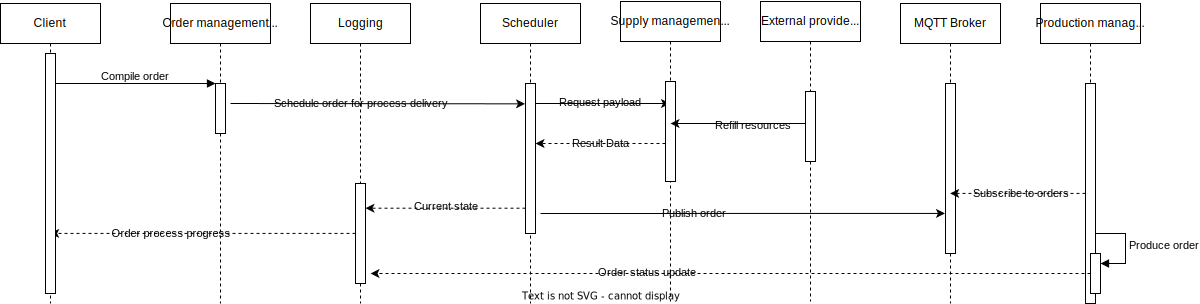
\includegraphics[width=1\linewidth]{diagrams/sequence-diagram.png}
    \caption{Sequence diagram}
    \label{fig:sequence-diagram}
\end{figure}

\section{Appendix B}

\begin{figure}[H]
    \centering
    \includegraphics[width=1\linewidth]{images/newman-test-report.png}
    \caption{Interoperability test results}
    \label{fig:interoperability-test}
\end{figure}

\vspace{12pt}
\end{document}
